\documentclass[12pt,addpoints]{exam}
\usepackage[utf8]{inputenc}
\usepackage[T1]{fontenc}
\usepackage[brazil]{babel}
\usepackage[a4paper, margin=2cm]{geometry}
\usepackage{graphicx, amsmath, amsfonts, amssymb, xcolor, url, tikz, pgfplots, subfigure}

\newcommand{\disciplina}{Laboratório de Princípios de Comunicações}
\newcommand{\periodo}{2023.1}
\newcommand{\avaliacao}{Guia de Experimentos 4}
\newcommand{\tema}{Modulação e Desmodulação em Ângulo.}
%\newcommand{\professor}{Bruno\ B.\ Albert e Edmar C.\ Gurjão}
%\newcommand{\professor}{Leocarlos B.\ S.\ Lima e Edson P.\ da Silva}
\newcommand{\professor}{Edson P.\ da Silva e Luciana Veloso}
%\newcommand{\professor}{Edmar C.\ Gurjão  e Luciana Veloso}
%\newcommand{\professor}{Bruno\ B.\ Albert e Edson P.\ da Silva}
%\newcommand{\professor}{Adolfo Herbster e Bruno Albert}
%\newcommand{\professor}{Edson Porto e Bruno Albert}

\pagestyle{head}
\firstpageheader{}{}{}
\runningheader{Lab.\ Princ.\ Comunicações}{\avaliacao}{Página \thepage}
\runningheadrule
\pointpoints{ponto}{pontos}
\newtheorem{exemplo}{Exemplo}[section]

\begin{document}
    
\noindent \includegraphics[height=2cm]{../Figuras/UFCGLogo.png} \hfill
\begin{minipage}{.66\textwidth} \large \centering \vspace{-1.8cm}
    Universidade Federal de Campina Grande -- UFCG \\
    Unidade Acadêmica de Engenharia Elétrica -- UAEE \\
    Curso de Graduação em Engenharia Elétrica
\end{minipage}
\hfill \includegraphics[height=2cm]{../Figuras/DEELogo.png} \\[12pt]

\noindent
\begin{tabular*}{\textwidth}{l @{\extracolsep{\fill}} r @{\extracolsep{6pt}} l}
    \textbf{\disciplina} && \\
    Período \periodo && \\
    \textbf{\avaliacao} && \\
    Tema(s): \tema && \\
    Professor(es): \professor && \\
\end{tabular*}
\noindent\rule[2ex]{\textwidth}{2pt}
    
\section{Introdução}

O presente guia descreve atividades experimentais a serem realizadas na disciplina Laboratório de Princípios de Comunicações do curso de graduação em Engenharia Elétrica da Universidade Federal de Campina Grande -- UFCG.

Os experimentos propostos deverão ser realizados no Laboratório de Princípios de Comunicações -- LPC, localizado na Central de Laboratórios da Unidade Acadêmica de Engenharia Elétrica da UFCG, empregando:
\begin{itemize}
    \item Computador com software GNU Radio Companion -- GRC (\url{http://gnuradio.org/}) instalado;
    \item Módulo USRP (do inglês \textit{Universal Software Radio Peripheral}) para transmissão e recepção de sinais numa abordagem conhecida como Rádio Definido por Software -- RDS.
\end{itemize}

Na seção \ref{sect:Preparacao} deste guia, propõe-se um conjunto de atividades de preparação a serem desenvolvidas pelo aluno antes da aula em que serão realizadas as práticas experimentais. Sem a realização prévia destas atividades pelo aluno, as práticas experimentais propostas ficarão comprometidas, tanto no tempo necessário para sua realização quanto no aproveitamento pelo aluno. Por essa razão, %\textbf{O aluno deverá realizar a Preparação na plataforma Moodle para ter acesso ao Relatório do Experimento}.
\textbf{o aluno só poderá realizar os experimentos em laboratório se apresentar ao professor no início da aula os resultados da preparação proposta}. 

% A aula terá duração de duas horas e o aluno deverá responder as questões do experimento que estão na parte final do guia, na atividade {\it Relatório do Experimento 4} na plataforma Moodle
A aula terá duração de duas horas e o aluno deverá entregar ao seu término, por escrito, respostas às questões referentes aos experimentos realizados propostas na Folha de Respostas (parte final do guia).

\section{Objetivos}

As práticas experimentais aqui propostas têm por objetivos:
\begin{itemize}
    \item Simular e analisar a modulação em ângulo;
    \item Simular e analisar o desmodulador FM;
\end{itemize}

\section{Preparação} \label{sect:Preparacao}

\subsection{Estudo}

Revise e pesquise sobre os conceitos:
\begin{itemize}
    \item Equivalência entre modulações PM e FM;
    \item Regra de Carson para os casos faixa larga e faixa estreita;
    \item Desmodulação FM usando a detecção por inclinação.
\end{itemize}

\subsection{Problemas}

Os problemas propostos a seguir devem ser obrigatoriamente resolvidos e apresentados por escrito ao professor antes do início das práticas de laboratório. Os resultados destes problemas serão necessários para a realização dos experimentos propostos. 

\begin{enumerate}
    \item Considere uma onda senoidal com amplitude de $1$~Vpp e período de $0,1$~ms como sinal de entrada para moduladores FM e PM, com constantes $K_f = 10^5$~Hz/V e $K_{p} = 10$~rad/V, respectivamente. Considere uma portadora de $100$~MHz com amplitude de $2$~Vpp.
    \begin{parts}
        \part Calcule o desvio de frequência $\Delta f_{\text{PM}}$, a razão de desvio $\beta_{\text{PM}}$ (também chamada de índice de modulação) e a largura de faixa estimada $B_{\text{PM}}$ para o caso PM.
        \part Calcule o desvio de frequência $\Delta f_{\text{FM}}$, a razão de desvio $\beta_{\text{FM}}$ (também chamada de índice de modulação) e a largura de faixa estimada $B_{\text{FM}}$ para o caso FM.
    \end{parts}
    \item Explique o que é e como funciona um VCO (\textit{Voltage Controlled Oscillator}). Explique como um VCO pode ser utilizado na geração de um sinal FM.    
    
    \item Mostre que a fase $\theta(t)$ do sinal PM $\varPsi(t) = A\cos[2\pi f_c t + \theta(t)]$ pode ser recuperada na saída do desmodulador coerente ilustrado na Fig.~\ref{fig:GRC_4-0}.
    
    \begin{figure}[h]
        \centering
        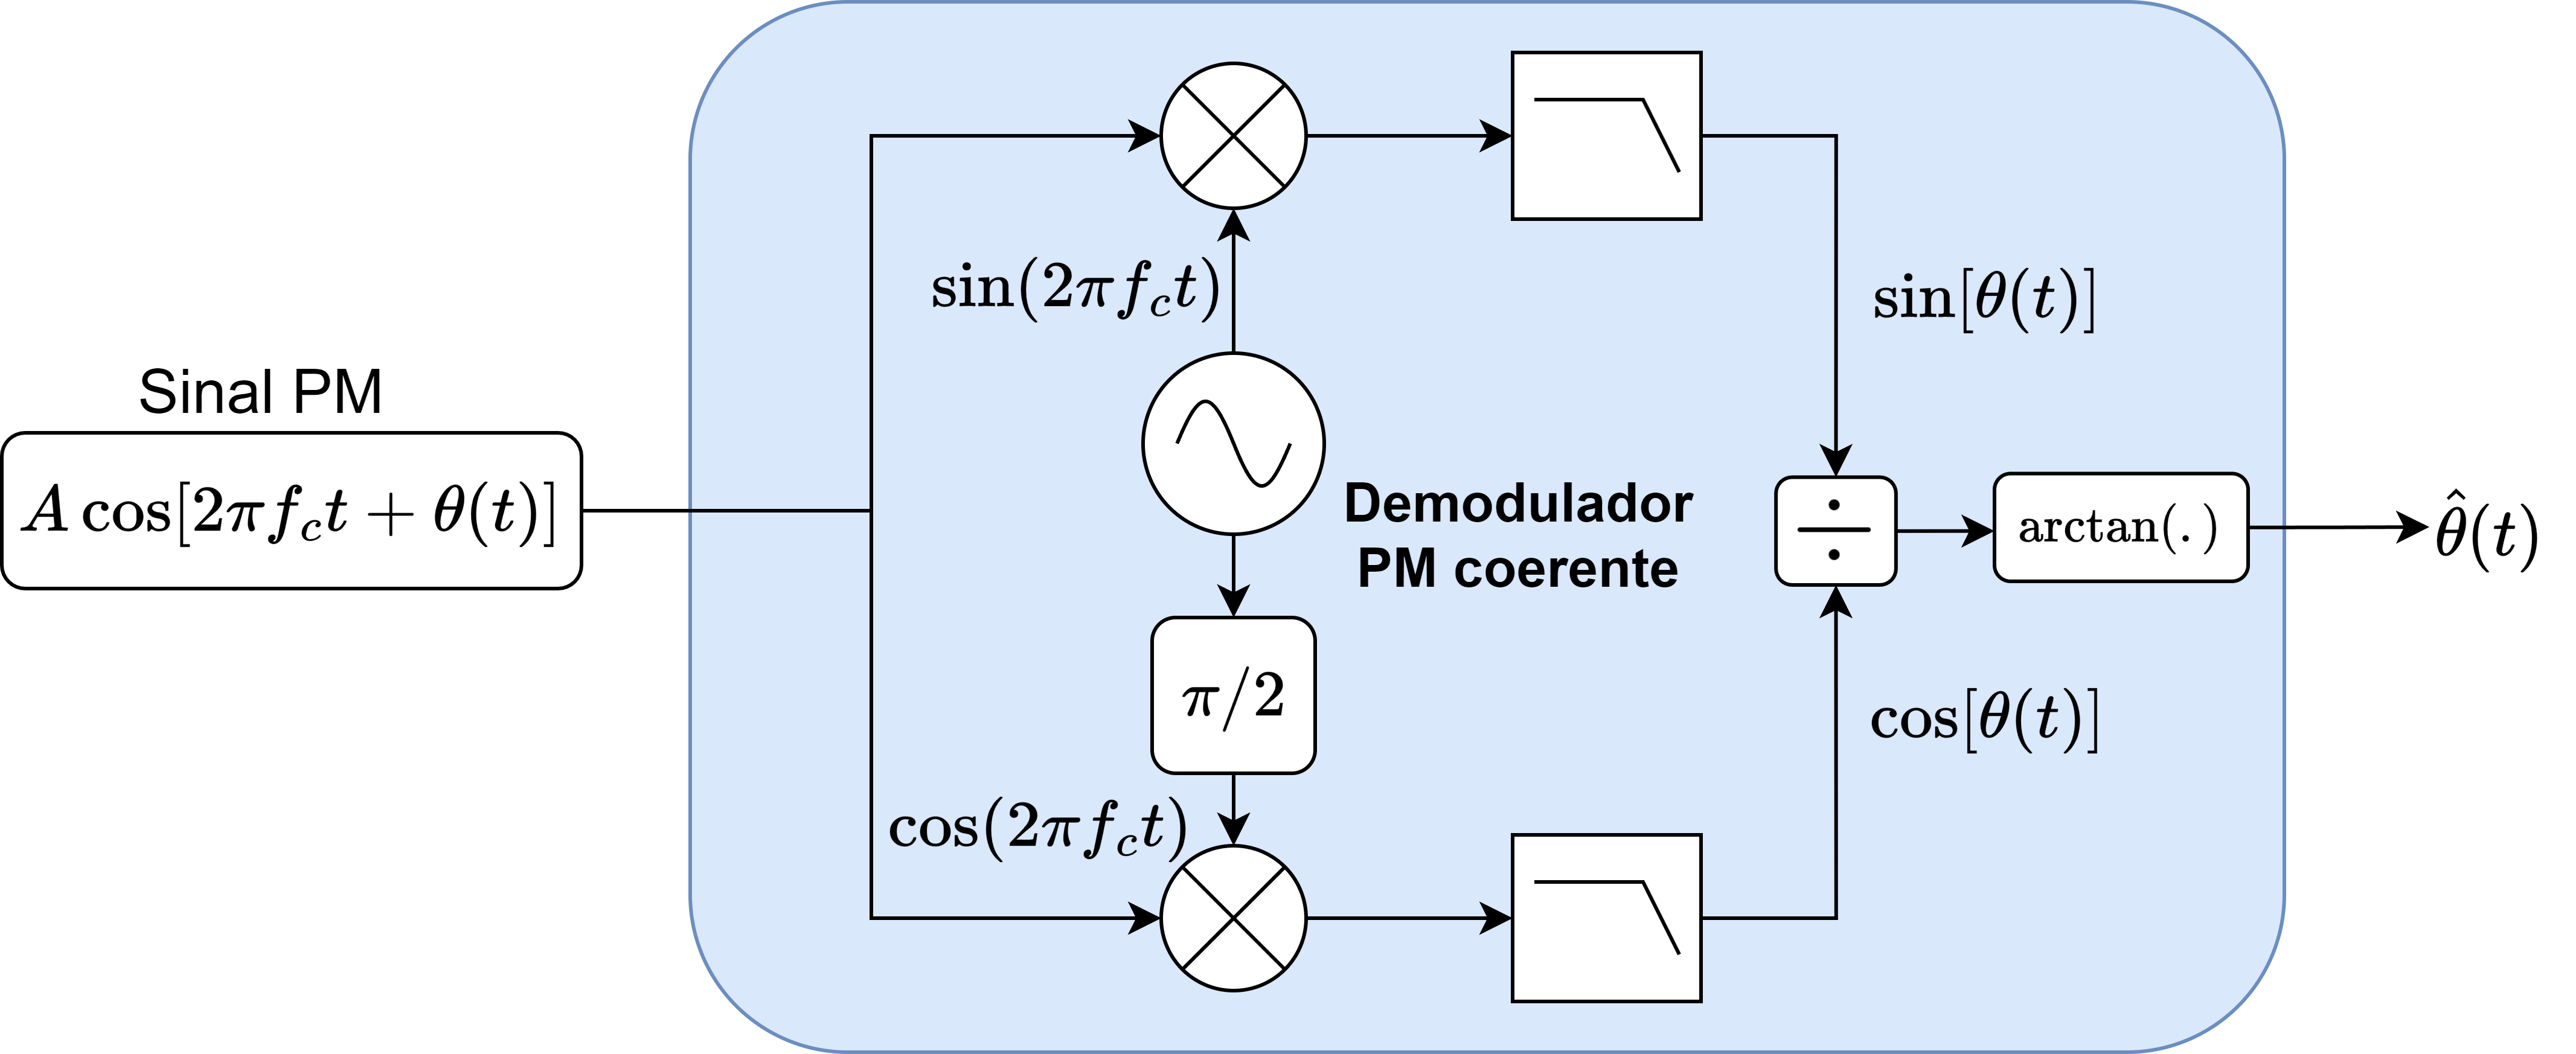
\includegraphics[width=0.85\linewidth]{./Figuras/PM-Demod.png}
        \caption{Diagrama de blocos de um desmodulador PM coerente.} 
        \label{fig:GRC_4-0}
    \end{figure}
  
  \end{enumerate}
  
\clearpage

\section{Experimentos}

A seguir são descritas práticas experimentais a serem realizadas no laboratório. 

\subsection{Experimento 1 -- Modulação PM com Detecção Síncrona}

O objetivo deste experimento é analisar as características da modulação PM.

\begin{enumerate}   
    \item Execute o software GRC e abra o arquivo \textbf{Labo4-1.grc}. A Figura \ref{fig:GRC_4-1} ilustra o diagrama deste experimento. Ele consiste na simulação da equação 
\begin{align}
  \varPsi(t) &= A\cos[2\pi f_c t + \Phi(t)[\nonumber\\
   &= A\{\cos(2\pi f_c t) \cos[\Phi(t)] -  \sin(2\pi f_c t) \sin[\Phi(t)]\}
  \label{eq:pm}
\end{align}
em que o $\Phi(t) = K_pm(t)$, de modo que $\varPsi(t)$ é um sinal PM ({\it Phase Modulation}), ou seja, uma portadora modulada em fase.
    \begin{figure}[htb]
        \centering
        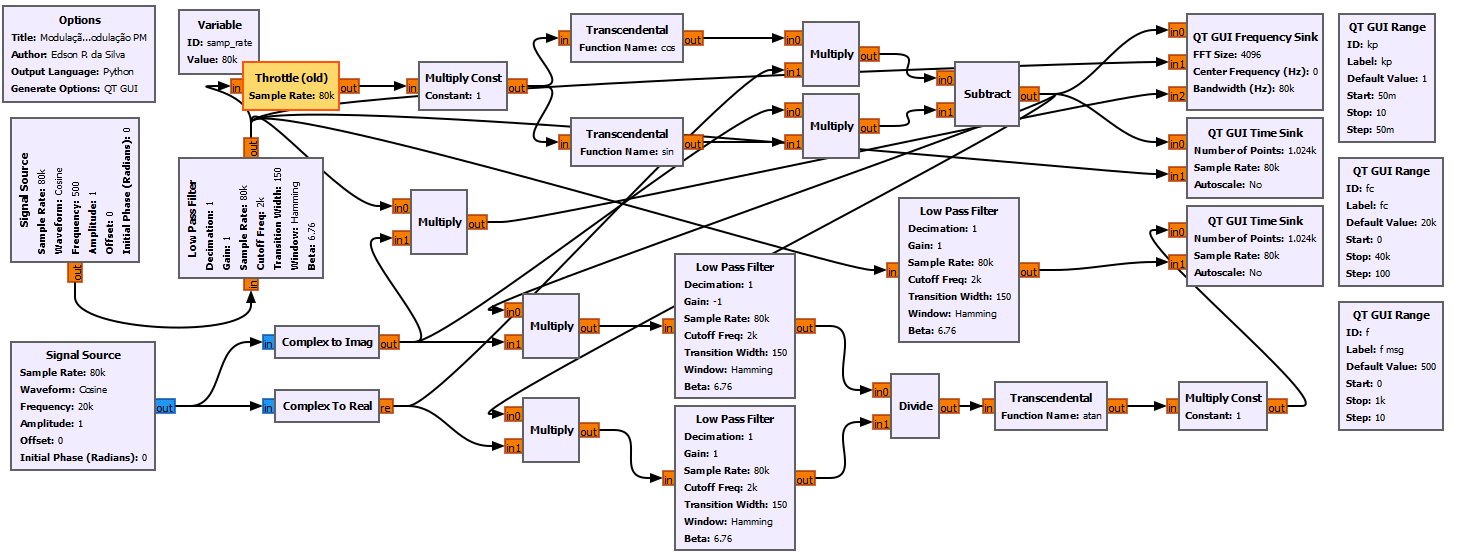
\includegraphics[width=0.95\linewidth]{./Figuras/Labo4-1.png}
        \caption{Diagrama de blocos para análise da modulação PM} 
        \label{fig:GRC_4-1}
    \end{figure}
  \item Execute o diagrama e responda às questões propostas na Folha de Respostas.
  \end{enumerate}
  
% \subsection{Experimento 1 -- Modulação PM de Faixa Estreita}

% O objetivo deste experimento é analisar a modulação PM em faixa estreita.

% \begin{enumerate}
%     \item Antes de iniciar as atividades com o GRC, crie uma pasta para guardar os arquivos de seus experimentos e copie nela os modelos de diagrama (arquivos .GRC) disponibilizados pelo professor para esta aula. \textbf{Não deixe de realizar isso, pois o computador deste laboratório não é para seu uso pessoal e os arquivos que você utilizará serão alterados por você durante o experimento};
%     \item Execute o software GRC e abra o arquivo \textbf{Labo4-1.grc}. A Figura \ref{fig:GRC_4-1} ilustra o diagrama deste experimento. Ele consiste na simulação da equação 
% \begin{equation}
%     \varPsi(t) \approx \cos\omega_ct - \Phi(t)\operatorname{sen}{\omega_{c}t}, \label{eq:pmnb}
% \end{equation}
% em que o $\Phi(t) = K_pm(t)$
%     \begin{figure}[htb]
%         \centering
%         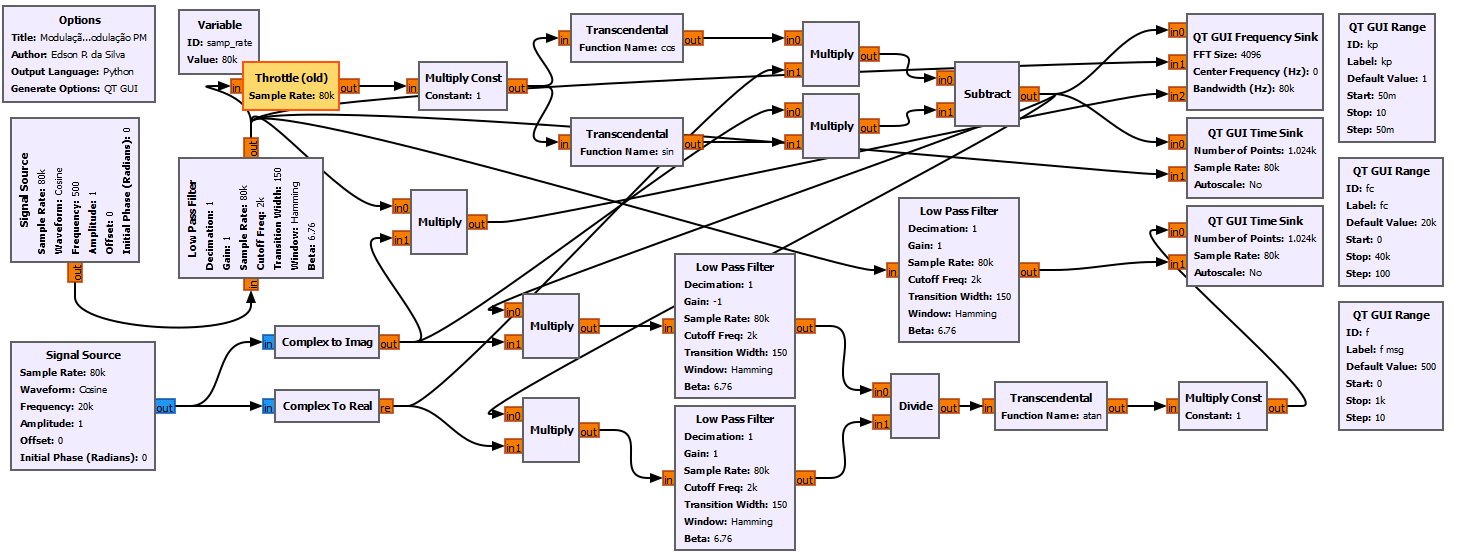
\includegraphics[scale=.5]{./Figuras/Labo4-1}
%         \caption{Diagrama de blocos para análise da modulação PM de faixa estreita.} 
%         \label{fig:GRC_4-1}
%     \end{figure}
%   \item Execute o diagrama e responda às questões propostas na Folha de Respostas.
% \end{enumerate}

\subsection{Experimento 2 -- Modulação FM}

O objetivo deste experimento é analisar o modulador FM de faixa larga. 

\begin{enumerate}
    \item Abra o arquivo \textbf{Labo4-2.grc} disponibilizado pelo professor. A Figura \ref{fig:GRC_4-2} ilustra o diagrama deste experimento. A modulação FM de faixa larga é obtida através de um VCO (Oscilador Controlado por Tensão, do inglês {\it Voltage Control Oscilator}).
    \begin{figure}[htb]
        \centering
        \includegraphics[scale=.5]{./Figuras/Labo4-2}
        \caption{Diagrama de blocos de um modulador FM de faixa larga usando um VCO.}
        \label{fig:GRC_4-2}
    \end{figure}
  \item Execute o experimento e observe a diferença em relação ao experimento anterior.
  \item Responda as questões propostas na Folha de Respostas.
\end{enumerate}

%\subsection{Experimento 3 -- Desmodulação com PLL}
%
%O objetivo deste experimento é observar desmodulação de sinais modulados em FM usando PLL ({\it Phase-Locked Loop})
%\begin{enumerate}
%    \item  Abra o arquivo \textbf{Labo4-3.grc} disponibilizado pelo professor. A Figura \ref{fig:GRC_4-3} ilustra o diagrama deste experimento. Ele consiste de um sistema de transmissão FM e recepção empregando um PLL como desmodulador; 
%    \begin{figure}[htb]
%        \centering
%        \includegraphics[scale=.5]{./Figuras/Labo4-3}
%        \caption{Diagrama de blocos de sistema de comunicação FM usando PLL na recepção.} 
%        \label{fig:GRC_4-3}
%    \end{figure}
%  \item Execute o experimento e responda as questões propostas na Folha de Respostas.
%\end{enumerate}
\newpage
\subsection{Experimento 3 -- Desmodulação com Detecção por Inclinação}

O objetivo deste experimento é mostrar o conceito de um receptor FM usando deteção por inclinação.

\begin{enumerate}
    \item  Abra o arquivo \textbf{Labo4-4.grc} disponibilizado pelo professor. A Figura \ref{fig:GRC_4-4} ilustra o diagrama deste experimento. Ele consiste de um sistema de transmissão FM e recepção empregando detecção por inclinação na desmodulação. Esse desmodulador consiste de um filtro passa-altas simulando a derivada do sinal modulado FM seguido por um detetor de envoltória.
    \begin{figure}[htb]
        \centering
        \includegraphics[scale=.5]{./Figuras/Labo4-4}
        \caption{Diagrama de blocos de sistema de comunicação FM usando detecção por inclinação na recepção.} 
        \label{fig:GRC_4-4}
    \end{figure}
  \item É mostrado o efeito do detector por inclinação para um sinal modulante dente de serra;
  \item Execute o experimento e responda as questões propostas na Folha de Respostas.
\end{enumerate}

% \subsection{Experimento 4 -- Receptor de sinal FM comercial}

% O objetivo deste experimento é ilustrar a recepção de sinal FM comercial empregando rádio por software (GNU Radio) e o módulo USRP.

% \begin{enumerate}
%     \item  Abra o arquivo \textbf{Labo4-5.grc} disponibilizado pelo professor. A Figura \ref{fig:GRC_4-5} ilustra o diagrama deste experimento. Ele consiste de um sistema de recepção de sinal FM comercial empregando um módulo USRP. 
%     \begin{figure}[htb]
%         \centering
%         \includegraphics[scale=.5]{./Figuras/Labo4-5}
%         \caption{Diagrama de blocos de receptor de sinal FM comercial empregando módulo USRP.} 
%         \label{fig:GRC_4-5}
%     \end{figure}
%     \item Na Figura \ref{fig:GRC_4-5}, o bloco \textbf{UHD: USRP Source} converte o sinal de frequência central e largura de faixa especificados nos parâmetros do bloco para seu equivalente passa-baixas. Observe que segue um filtro passa-baixas com frequência de corte igual à metade da largura de faixa do sinal FM sintonizado no bloco \textbf{UHD: USRP Source};
%     \item O bloco \textbf{WBFM Receive} implementa a desmodulação do sinal FM a partir do equivalente passa-baixas do sinal modulado FM;
%     \item Execute o experimento e responda as questões propostas na Folha de Respostas.
% \end{enumerate}

\newpage \clearpage \pagenumbering{arabic}

\noindent \includegraphics[height=2cm]{../Figuras/UFCGLogo} \hfill
\begin{minipage}{.66\textwidth} \large \centering \vspace{-1.8cm}
    Universidade Federal de Campina Grande -- UFCG \\
    Unidade Acadêmica de Engenharia Elétrica -- UAEE \\
    Curso de Graduação em Engenharia Elétrica
\end{minipage}
\hfill \includegraphics[height=2cm]{../Figuras/DEELogo} \\[12pt]

\noindent
\begin{tabular*}{\textwidth}{l @{\extracolsep{\fill}} r @{\extracolsep{6pt}} l}
    \textbf{\disciplina} && \\
    Período \periodo && \\
    \textbf{\avaliacao\ -- Folha de Respostas} && \\
    Tema(s): \tema && \\
    Professor(es): \professor && \\[12pt]
    \textbf{Aluno:} \hrulefill & \textbf{Data:} \makebox[3cm]{\hrulefill} & \\
\end{tabular*}
\noindent\rule[2ex]{\textwidth}{2pt}

\section*{Experimento 1 -- Modulação PM com Detecção Síncrona}

\begin{questions}
    \question Quais as diferenças mais visíveis entre o sinal PM e o sinal AM-DSB-SC no domínio da frequência? E no domínio do tempo?
    \fillwithlines{1.5in}
    \question Estime o desvio de frequência $\Delta f$ e a largura de faixa $B_{\text{PM}}$ do sinal modulado usando os gráficos no tempo e na frequência. Qual a razão de desvio $\beta$?
    \fillwithlines{0.75in}
    
    \question Observando o espectro dos sinais, descreva qualitativamente a relação que existe entre a variação no valor de $K_{p}$ e a largura de banda da portadora modulada.
    \fillwithlines{1.0in}
     
    \question Observe as formas de onda no domínio do tempo do sinal mensagem e do sinal desmodulado. Para que intervalo de valores de $K_p$ o sinal mensagem é recuperado sem distorção? Acima de um determinado valor limiar de $K_p$ o sinal desmodulado sofre distorções. O que explica esse fenômeno?
    \fillwithlines{1.50in}


    
%    \fillwithlines{0.5in}
%    \question Varie a frequência da portadora $f_c$ para 20 kHz e observe que isso não altera a largura de faixa do sinal PM. Altere a frequência da fonte para 1 kHz e explique o que ocorreu com a largura de faixa do sinal modulado em fase, $B_{PM}$. A razão de desvio $\beta$ se altera?
%    \fillwithlines{0.5in}
    
%    \question Quando temos um $K_{p} < 0.5$ o sinal PM é considerado de faixa estreita e pode ser aproximado pela equação
%    \begin{equation}
%      \varPsi(t) \approx A(\cos\omega_ct - \Phi(t)\operatorname{sen}{\omega_{c}t}),
%      \label{eq:pmnb}
%\end{equation}
%em que o $\Phi(t) = K_pm(t)$. Esse sinal é semelhante a um sinal AM e foi usado para se obter um sinal FM faixa larga, usando multiplicadores de frequência. Faça $K_{p} = 0.3$ e estime a largura de faixa do sinal PM e a nova razão de desvio $\beta$.
%    \fillwithlines{0.5in}
%    
    % \question Deixe a frequência da fonte em $500$~Hz. Varie agora a frequência da portadora. Observe no gráfico no domínio da frequência que o sinal mensagem é deslocado para frequência da portadora. Coloque a portadora em 15 kHz. Houve alteração na largura de faixa do sinal PM? A razâo de desvio $\beta$ se altera?
    % \fillwithlines{1.25in}
\end{questions}
% \section*{Experimento 1 -- Modulação PM de Faixa Estreita}

% \begin{questions}
%     \question Observe que o sinal no tempo tem uma variação na amplitude e, portanto, não pode ser considerado uma modulação PM. Quais as amplitudes dos impulsos em 9.5 kHz, 10 kHz e em 10,5 kHz (em dB)? Qual a largura de faixa do sinal modulado? Qual a razâo de desvio (índice de modulação) $\beta$? Considere que $K_p$ é dado em rad/Hz.
%     \fillwithlines{1.25in}
%     \question Varie a constante do modulador PM, $K_{p}$, de modo que o sinal modulado possa ser considerado um PM de faixa estreita. Qual é esse valor? Qual a nova razâo de desvio (índice de modulação) $\beta$? Observe que quando diminuímos $K_{p}$ o sinal mensagem diminui de amplitude. Quais as novas amplitudes dos impulsos 9.5 kHz, em 10 kHz e em 10,5 kHz? A largura de faixa do sinal modulado se alterou?
%     % Quais são o desvio de frequência $\Delta f$, a razão de desvio $\beta$ e a largura de faixa $B_{\text{PM}}$ (não esqueça as unidades) do sinal modulado nesse caso?
%     \fillwithlines{1.25in}
    
%     % \question Faça $K_{p} = 0.2$. Varie a frequência da fonte para 200~Hz e, em seguida, para 1~kHz. Observe o gráfico no domínio da frequência. Quais as novas larguras de faixa para cada frequência da fonte acima, medindo no gráfico? Observe a Eq.~\ref{eq:pmnb} e explique porque a amplitude da portadora e das bandas laterais não se alteram?
%     % \fillwithlines{1.25in}

%     \question Varie a frequência da fonte para 800 Hz e explique o que ocorreu com a largura de faixa do sinal modulado em fase, $B_{PM}$. Observe que as amplitudes da portadora e das bandas laterais não se alteram. A razâo de desvio $\beta$ se altera?
%     \fillwithlines{1.25in}
    
%     % \question Varie a frequência da fonte e explique o que ocorreu com a largura de faixa do sinal modulado em fase, $B_{PM}$. Observe que as amplitudes da portadora e das bandas laterais não se alteram. A razâo de desvio $\beta$ se altera?
%     % \fillwithlines{1.25in}
    
%     % \question Deixe a frequência da fonte em $500$~Hz. Varie agora a frequência da portadora. Observe no gráfico no domínio da frequência que o sinal mensagem é deslocado para frequência da portadora. Coloque a portadora em 15 kHz. Houve alteração na largura de faixa do sinal PM? A razâo de desvio $\beta$ se altera?
%     % \fillwithlines{1.25in}
% \end{questions}

\section*{Experimento 2 -- Modulação FM}

\begin{questions}
    \question Faça uma estimativa do desvio de frequência observando o gráfico no tempo (maior e menor período). 
    \fillwithlines{0.25in}
    
    \question Qual a constante do modulador FM $K_{f}$ e o índice de modulação $\beta$? Considere a largura de faixa da onda quadrada de entrada até a quinta harmônica. Compare $K_{f}$ com o parâmetro {\it Sensitivity} do VCO.
    \fillwithlines{0.5in}
    
    \question Qual a largura de faixa do modulador FM calculada pela regra de Carson e a largura de faixa observada no espectro em frequência (considere as componentes de frequência até a quinta harmônica na observação a partir dos picos)?%redução de aproximadamente 10 dB sobre as de maior potência)?
    \fillwithlines{0.25in}
    
    \question Alterar a frequência da portadora altera a largura de faixa do modulador FM? E quanto à frequência do sinal modulante?
    \fillwithlines{0.5in}
    
    \question Altere a amplitude do sinal modulante para $1,5$. Qual a nova largura de faixa do sinal modulado pela regra de Carson e observando-se o espectro de frequência, considerando $K_{f} = 10^{4}$~Hz/V?
    \fillwithlines{0.25in}
    
    % \question Coloque uma onda quadrada como sinal de entrada e execute o experimento. Observe que há apenas duas frequências no sinal modulado (no tempo). Qual seria, então, o desvio de frequência nesse caso, observando o gráfico no tempo? E utilizando a teoria?
    % \fillwithlines{0.25in}
\end{questions}

%\section*{Experimento 3 -- Desmodulação com PLL}
%
%\begin{questions}
%    \question Observe que o sinal desmodulado apresenta um ``ruído''. Coloque um filtro passa-baixas para atenuar o ruído. Qual a frequência de corte que você usou para isso? 
%    \fillwithlines{0.25in}
%    
%    \question Troque o sinal de entrada por um dente de serra. Qual a frequência de corte do filtro adequada nesse caso? Justifique sua resposta.
%    \fillwithlines{0.5in}
%\end{questions}

\section*{Experimento 3 -- Desmodulação com Detecção por Inclinação}

\begin{questions}
    \question Observe que o sinal na saída do derivador (bloco {\em High Pass Filter}) está modulado em amplitude e também em frequência. Qual o índice de modulação do sinal AM? Mude a amplitude do sinal modulante para cima e para baixo, para se obter um índice de modulação 0,5 e 1,0. Quais são esses valores de amplitude? % O que ocorre com a largura de faixa do sinal FM, para os dois casos em relação à amplitude de 0,2?
    \fillwithlines{1in}

%    \question Se usássemos um oscilador local para detetar, o sinal da saída do derivador, como no caso de um detetor síncrono para um sinal AM. Qual seria a frequência desse oscilador local? Justifique.
%    \fillwithlines{1in}

\end{questions}

% \section*{Experimento 4 -- Receptor de sinal FM comercial}

% \begin{questions}
%     \question Altere a largura de faixa de recepção alterando o valor na parte inferior da janela do gráfico da FFT. Experimente aumentá-la até incluir estações FM vizinhas, ou diminuí-la significativamente. Explique o efeito observado.
%     \fillwithlines{1in}
    
% \end{questions}

\end{document}
